\documentclass[a4paper]{article}
\usepackage{iwslt15,amssymb,amsmath,epsfig}
\usepackage{csquotes}
\usepackage{algorithm}
\usepackage{listings}
\lstset{
     breaklines=true,
     basicstyle=\ttfamily
}

\setcounter{page}{1}
\sloppy		% better line breaks
%\ninept

\newcommand{\ts}{\textsuperscript}

\title{Hand Gesture Recognition with Convolutional Neural Networks}

%%%%%%%%%%%%%%%%%%%%%%%%%%%%%%%%%%%%%%%%%%%%%%%%%%%%%%%%%%%%%%%%%%%%%%%%%%
%% If multiple authors, uncomment and edit the lines shown below.       %%
%% Note that each line must be emphasized {\em } by itself.             %%
%% (by Stephen Martucci, author of spconf.sty).                         %%
%%%%%%%%%%%%%%%%%%%%%%%%%%%%%%%%%%%%%%%%%%%%%%%%%%%%%%%%%%%%%%%%%%%%%%%%%%
\makeatletter
\def\name#1{\gdef\@name{#1\\}}
\makeatother
\name{{\em Benjamin Alt, Lukas Hennig, Felix Hertlein}}
%%%%%%%%%%%%%%% End of required multiple authors changes %%%%%%%%%%%%%%%%%

\address{Interactive Systems Lab, Institute for Anthropomatics and Robotics\\
Karlsruhe Institute of Technology, Germany\\
{\small \tt benjamin.alt@student.kit.edu}\\
{\small \tt lukas.hennig@student.kit.edu}\\
{\small \tt felix.hertlein@student.kit.edu}
}
%
\begin{document}
\maketitle
%
\begin{abstract}
TODO
\end{abstract}

\section{Introduction}
TODO

\section{Dataset}
TODO

\section{Models}
TODO

\section{Evaluation}
\subsection{Validation on custom dataset}
\begin{figure}[t]
     \centering
     \begin{tabular}{ccc}
          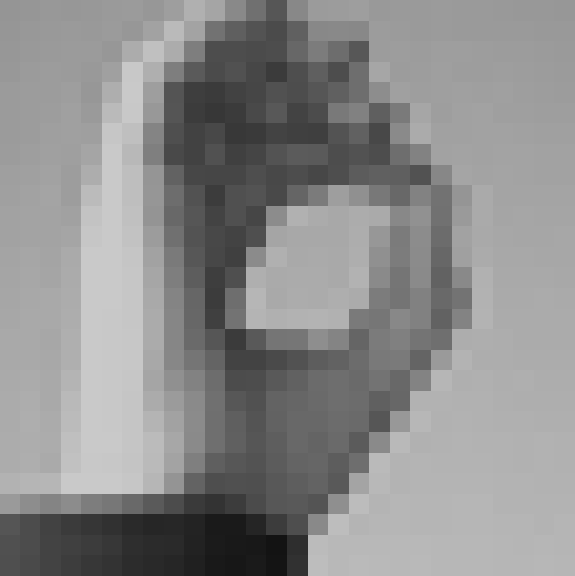
\includegraphics[width=.25\linewidth]{graphics/custom_dataset/orig0}&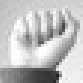
\includegraphics[width=.25\linewidth]{graphics/custom_dataset/orig1}&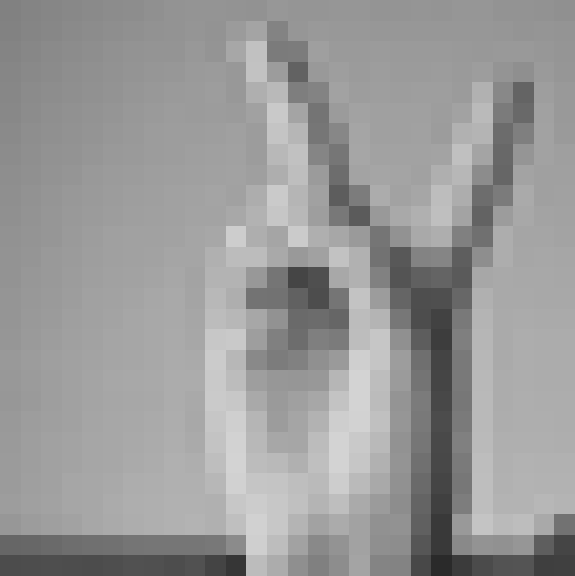
\includegraphics[width=.25\linewidth]{graphics/custom_dataset/orig2} \\
          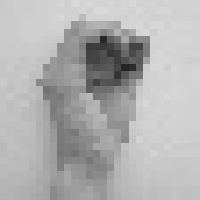
\includegraphics[width=.25\linewidth]{graphics/custom_dataset/custom0}&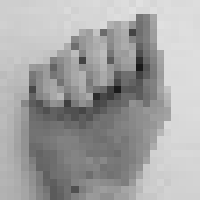
\includegraphics[width=.25\linewidth]{graphics/custom_dataset/custom1}&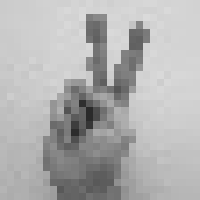
\includegraphics[width=.25\linewidth]{graphics/custom_dataset/custom2}
     \end{tabular}
     \caption{\textit{Exemplary images from original (top row) and custom (bottom row) datasets.}}
     \label{fig:custom_dataset} 
\end{figure}
To determine the trained model's capacity to generalize to real-world examples beyond those of the provided test set, we created a small custom dataset of 60 images of sign language gestures made by our own hands in front of a white background. To keep the scenario as realistic as possible, preprocessing of the images was constrained to grayscale conversion, cropping and rescaling to the expected size of 28x28 pixels. Three of the images in the custom dataset, together with corresponding images from the provided test set, are shown in figure \ref{fig:custom_dataset}. Despite its capability of correctly classifying every image in the provided test set, the model failed to correctly classify a single image from the custom dataset. The poor performance of the classifier on real-world data indicates that the model did not learn salient features for classifying ASL hand gestures in general, but instead learned features only relevant to these particular training and test sets. To test this hypothesis, we we chose to generate human-interpretable visual representations of the learned features. In the literature, several approaches for visualizing the features learned by neural networks in general and convolutional neural networks in particular have been proposed [TODO: CITATION]. PyTorch implementations of multiple neural network visualization algorithms are provided in the repository \textit{pytorch-cnn-visualizations} [TODO: CITATION], from which we used and slightly adapted the visualization of convolutional filters described in section \ref{sec:filter_visualization} as well as the gradient class-activation mapping (GradCAM) shown in section \ref{sec:gradcam}.

\subsection{Visualization of filters}
\label{sec:filter_visualization}
\begin{figure}[t]
     \centering
     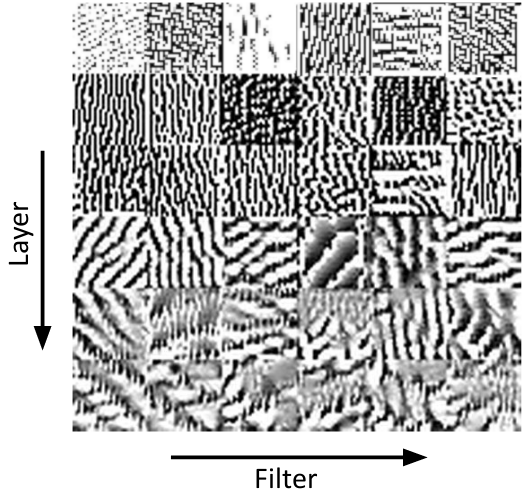
\includegraphics[width=.9\linewidth]{graphics/filters}
     \caption{\textit{Input images optimizing convolution outputs for the filters of the six convolutional layers of the final model. Only a subset of all layers of each filter is shown.}}
     \label{fig:filters}
\end{figure}
A common visualization technique for understanding the features learned by a convolutional neural network is to display the weights in the filters of the convolutional layers [TODO: CITATION]. Filters at the first layers tend to be easily interpretable, usually as pattern or edge detectors, while the filters of deeper layers become less interpretable. A different approach is to visualize the optimal input image with respect to a given convolution. This way, we do not visualize the weights, but rather the \enquote{archetypical feature} which maximizes the output of a given filter. Algorithm \ref{alg:filter_visualization} shows a PyTorch-based implementation of the optimization-based filter visualization.

\begin{algorithm}
     \caption{Convolution Input Optimization}\label{alg:filter_visualization}
     \begin{lstlisting}[language=Python]
hook_pytorch_layer(model)
x = random_tensor(shape=(224, 224, 3))
optimizer = torch.optim.Adam([x])
for i in range(30):
  optimizer.zero_grad()
  for j, layer in enumerate(model):
    x = layer(x) # forward pass
    if j == selected_layer:
      break # forward hook function has been triggered
    loss = -torch.mean(conv_output)
    loss.backward()
    optimizer.step()
     \end{lstlisting}
\end{algorithm}

A PyTorch layer hook function is registered to save the output (here: \texttt{conv\_output}) of the convolution with a specified filter at a specified layer (here: \texttt{selected\_layer}). An \texttt{Adam} optimizer [CITATION] is initialized for a random image. In each of a total of 30 iterations, the optimizer's gradients are reset and the current version of the input image is forward-propagated through the network up to the specified layer, at which point the registered hook function stores the convolution output in \texttt{conv\_output}. The loss (the negative mean of \texttt{conv\_output}) is then backpropagated through the network and the image is updated by the optimizer.\\
A subset of the resulting images are shown in figure \ref{fig:filters}. In the first layers, the outputs of the convolutions are maximized for high-frequency inputs with different primary orientations. Filters in deeper layers respond more strongly to lower-frequency patterns. This indicates that filters in deeper layers respond more strongly to larger features of the image and suggests that the network has learned to extract features beyond the high-frequency noise characteristics of the training set.

\subsection{GradCAM visualization}
\label{sec:gradcam}
\begin{figure}[t]
     \centering
     \begin{tabular}{ccc}
          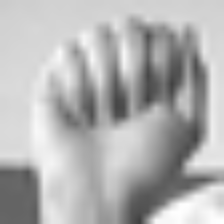
\includegraphics[width=.25\linewidth]{graphics/gradcam/layer1/0_original}&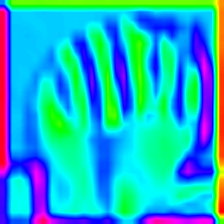
\includegraphics[width=.25\linewidth]{graphics/gradcam/layer1/0_map}&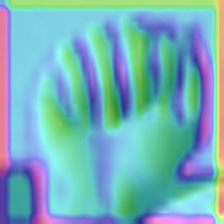
\includegraphics[width=.25\linewidth]{graphics/gradcam/layer1/0_overlaid} \\
          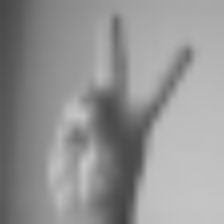
\includegraphics[width=.25\linewidth]{graphics/gradcam/layer3/0_original}&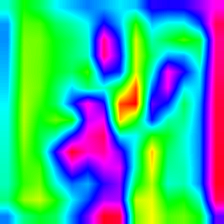
\includegraphics[width=.25\linewidth]{graphics/gradcam/layer3/0_map}&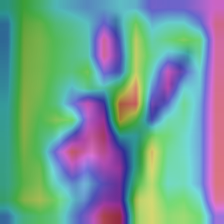
\includegraphics[width=.25\linewidth]{graphics/gradcam/layer3/0_overlaid} \\
          
\includegraphics[width=.25\linewidth]{graphics/gradcam/layer6/1_original}&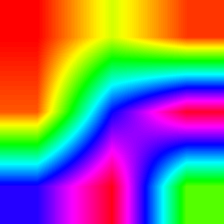
\includegraphics[width=.25\linewidth]{graphics/gradcam/layer6/1_map}&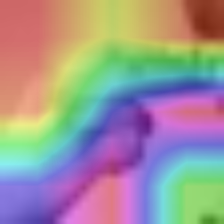
\includegraphics[width=.25\linewidth]{graphics/gradcam/layer6/1_overlaid} \\
          \textit{(a) Original} & \textit{(b) GradCAM} & \textit{(c) Overlaid}
     \end{tabular}
     \caption{\textit{GradCAM visualization of learned features for convolutional layers 1, 3 and 6 (1\ts{st}, 2\ts{nd} and 3\ts{rd} row respectively). The visualizations in column (c) are produced by overlaying the original image (a) with its GradCAM (b).}}
     \label{fig:gradcam}
\end{figure}
While the visualizations of optimal convolution inputs of section \ref{sec:filter_visualization} indicate that the network learned something other than noise, it does not give any indication whether the learned features are meaningful in the context of hand gesture recognition. To that end, we used the gradient class-activation mapping (GradCAM) algorithm which generates a heat map indicating the importance of every pixel in the classification of an image. Unlike the generic visualization of optimal convolution inputs above, GradCAM is \textit{class-discriminative}: It visualizes how much a each pixel contributed to the model's decision to classify an image into a particular class. Consequently, for an image of the gesture for the letter \enquote{A}, we expect the gradient class-activation map to highlight different regions of the hand than for an image of the gesture for the letter \enquote{V}, because different parts of the hand carry the salient information: The \enquote{A-ness} of an image of a hand is mainly captured by the four parallel fingers curled into a fist, while the \enquote{V-ness} of an image of a hand is mainly determined by the positions of the tips of the index and middle fingers.\\
\begin{algorithm}
     \caption{Gradient Class-Activation Mapping}
     \label{alg:gradcam}
     \begin{enumerate}
          \item Compute the gradient $\frac{\partial y^c}{\partial A^k}$ of the class score $y^c$ for class $c$ with respect to the feature maps $A^k$ of the given convolutional layer
          \item Compute the \textit{neuron importance weights}\\ $\alpha^c_k = \frac{1}{Z} \sum_i \sum_j \frac{\partial y^c}{\partial A^k_{ij}}$
          \item Compute the class-discriminative localization map\\
          $L^c_{GradCAM} = ReLU(\sum_k \alpha_k^c A^k)$
     \end{enumerate}
\end{algorithm}
Algorithm \ref{alg:gradcam} summarizes the GradCAM algorithm. Note that the neuron importance weights $\alpha_k^c$ are the result of global average pooling of the gradients and encode the importance of feature map $A^k$ for the decision for class $c$. $Z = i*j$ denotes the size of the feature map. The ReLU activation of the weighted sum in the third step is required to only keep pixels whose intensity should be \textit{increased} to increase $y^c$.\\
Exemplary results of computing the gradient class-activation maps for images from the test dataset are shown in figure \ref{fig:gradcam}. It is noteworthy that the size of the considered regions increases with the depth of the layers. In layers 3 and 6, the salient features (the fingertips for the \textit{V}, the orientation of the fingers for the \textit{H}) are captured. The first row of figure \ref{fig:gradcam} shows that in the first layer, edges are primarily considered, which is expected. However, only dark edges on the right side of the fingers are highlighted. This indicates that the network at least partially learned to consider the lighting characteristics of the image in the first layers, which is problematic because the hands in the images of the provided training and test sets are illuminated exclusively from the left. Real-world examples such as our custom dataset will not necessarily share these lighting characteristics. This supports our hypothesis that the uniformity of the training and test sets prevents the model from generalizing well to real-world examples.

\section{Conclusion and outlook}
Considering the implementation and evaluation of our model, a number of relevant conclusions can be drawn.\\
First, it is interesting to observe that for this particular problem, test accuracies exceeding [TODO]\% can be reached with a very simple neural network consisting of only one convolutional layer and two linear layers without regularization. With a relatively simple deep model containing three convolutional and three fully connected layers, test accuracies exceeded [TODO]\% without any optimizations. This illustrates the particular suitability of convolutional neural networks for image classification in general as well as the suitability of the architecture combining convolutional feature extractors and fully connected classifiers for the particular task of hand gesture recognition.\\
Second, we observed that while a high-performing network architecture and parameterizion could be found relatively quickly, a large amount of fine-tuning both of the architecture and the parameters was required to reach test accuracies exceeding 98\%. Somewhat surprisingly, grid search proved to be less effective in maximizing test accuracy than manual parameter tuning due to the high dimensionality of the parameter space. State-of-the-art approaches for automatic architecture and parameter search solve this problem by leveraging reinforcement learning \cite{Zoph2016}, dimensionality reduction \cite{Hinz2018} or massive parallelization \cite{Li2018}.\\
Lastly, and probably most significantly, we observed that the capacity of the trained model to generalize to test instances from different distributions at least partly depends on the variance of the training set. In our case, the fact that the training dataset featured only seven different hands and was generated by data augmentation from only 1704 original images, all of which share very similar backgrounds and lighting characteristics, caused the network to learn at least some characteristics of the dataset irrelevant for the actual classification of hand gestures, despite heavy regularization efforts and additional data augmentation during training. Along the same lines, we observed that a high classification accuracy on the test set is not a measure of true generalization capacity if the test set is drawn from the same or a very similar distribution as the training set.\\
\subsection{Future work}
Several approaches can be taken to improve the generalization capacity of our model. First, the neural network architecture can be modified to increase, instead of decrease, the filter size in deeper layers [TODO: Why would we want this exactly?] Second, the very high dropout probability of our network could likely be reduced, which would then permit a smaller network size and consequently, by the reduced number of parameters, would be less likely to overfit on the particularities of the training (and test) datasets. Third, the variance of the training data could be increased either by incorporating a larger custom dataset into the training data or by more aggressive data augmentation.

% \bibliographystyle{IEEEtran}
% \begin{thebibliography}{10}
% \bibitem[1]{ES1} Smith, J. O. and Abel, J. S., 
% ``Bark and {ERB} Bilinear Transforms'', 
% IEEE Trans. Speech and Audio Proc., 7(6):697--708, 1999.  
% \bibitem[2]{ES2} Lee, K.-F., Automatic Speech Recognition: 
% The Development of the 
% SPHINX SYSTEM, Kluwer Academic Publishers, Boston, 1989.
% \bibitem[3]{ES3} Rudnicky, A. I., Polifroni, Thayer, E. H.,
%  and Brennan, R. A.  
% "Interactive problem solving with speech", J. Acoust. Soc. Amer., 
% Vol. 84, 1988, p S213(A).
% \end{thebibliography}
\end{document}

